% !TEX root = ../thesis.tex
\chapter{Recommendation system state of the art}
\label{chapter:<recommendation_system_state_of_the_art>}

\section{Introduction}

This chapter will simply expose to the reader some backgrounds about recommendation systems. Basic concepts of recommendation systems, its algorithms, explanations and layouts might be of knowledge of the one in hand of this project description, but a brief review could be useful to understand the whole application design. The state of the art of a recommendation system is also analyzed in order to give to the reader a meaningful idea of that a recommendation system is supposed to work and reach its goals in the optimal way. 

With the emerging of hardware resources and computational power recommendation system have grown and diversified. Just decades ago a recommendation would have taken hundreds of mainframes to be completed. Nowadays with hardware as a commodity and all the emerging cloud solutions that allows to have the amount of desired computational power, RAM and storage for just the time requested, deploying recommendation system has never been faster and cheaper. Also big companies like Netflix completely run on cloud systems like the one by Amazon or Rackspace. 
As soon as internet and computers evolved and more information was available and interconnected, search engine started to arise and being adopted by the newborn internet community. These early search engines were basically of two types \cite{spiegazione_confidenza_raccomandazione}:

\begin{itemize}
\item \textbf{Information retrieval}. A keyword is the base concept of this type. Keyword or a set of keywords are used to look for the desired content. The points of failure of this kind of search may be the chosen keyword. In fact the content could have been categorized used a set of different keywords that the one the user is looking for, thus the content is not selected even if it is relevant to the user.
\item \textbf{Information filtering}. Preferences established by the user are used as a background knowledge to select the relevant items for the user or, alternatively, properties of a item or a subset of items can be used to lead to another set of relevant items.
\end{itemize}

Recommendation systems are basically of the second type or information retrieval and they evolved heavily under all the 90'. Nowadays search engine giants like Google or Yahoo use both types in integrated system to lead to stronger and valuable results. Lately with the adoption of smart phones and tablets which have a small screen size and different human-computer interaction than a traditional personal computer with a mouse and a keyboard, recommendation systems to surf content on those devices are critical applications and under heavily development. 

Recommendation system are widely adopted in all the most known website and web applications. They may be based on:

\begin{itemize}
\item \textbf{User profile}: the recommendation is based on information gathered from the user. The information can be explicit or implicit. An example of explicit information is the set of ratings. Supposing we are in the case of a movie web application the user profile is the list of all the ratings that the user made for each movie in the database. An example of implicit is the set of pages or items that the user viewed, in the case of a movie web application this can be just the list of items that the user viewed during the continuous navigation of the website.
\item \textbf{Item content}: the recommendation is based on the current item or set of item displayed. In this case no information about the user is used by the algorithm. As and example of this scenario for a web application abut movies, the item content for the recommendation can be the name of the actors, the genre, the release date or the plot description.
\end{itemize}

The reader should see a recommendation system as a complementary system of a search engine and not a different implementation of a concept of a search engine. They solve two different problems. Search engines are really powerful when the user knows or has an idea of what he or she is looking for. The user types a keyword or a set of keyword in a text field and the algorithms involved select the contents relevant for that search.

Recommendation system are useful when the user actually does not know what she or he is looking for. Their added value is in suggesting an item that may be interesting from the user perspective. The user has not a keyword to start his/her navigation with. The user will just receive the new item, maybe without even asking about it. Since search engines and recommendation systems solve different problems they are often implemented one aside the other to keep the user in the web application or to satisfy user's needs. From a research \cite{usercentric_evaluation_framework} at RecSys \cite{recsys}, 45\% of users will likely shop in a web application that employs recommendation technology and 69\% of users in the highest spending category are more likely to desire the support of recommendation technology during their web application navigation or shopping. So recommendation systems are valuable from both user and web application. It offers the benefit of an easy way to navigate and find items for an user and a better service and/or a better shopping experience for the web application.

\section{Analysis}
\label{sec:Analysis}

Recommendation systems, like search engines, are very complex systems with a strong time constraints. From a recent study \cite{page-abandonment} users often leave web pages in 10-20 seconds but pages with a clear value proposition can hold people's attention for much longer because visit-durations follow a negative Weibull distribution. Due to this nature of the web user pages should load as quick as possible and thus search results or recommendation results should be displayed in no more than few seconds or the user will leave the page without even looking at the results. These kind of constraints have influenced the way recommendation systems have been developed and evolved through time.
From a black box point of view a recommendation system is just a tool that given the proper input returns an output. No matter which algorithm, programming language, or added feature the recommendation system applies, all recommendation system analyzed respect this constraint. Given that we will explore the input of a recommendation system and its stack. The algorithms can be categorized in two families depending from the requested input:

\begin{itemize}
\item \textbf{Content based}. The elaboration of the suggested items listed are based on the content of the available object options \cite{content-based-recommendation-systems}. Therefore the only needed input for this family of algorithms is the \ac{ICM}. Due to the fact that these algorithms do not know anything about the user they are exposed to some limitations:

  \begin{itemize}
  \item \textit{the list of metadata influences the recommendation directly}. If the list of metadata is not selected properly the recommendation can lead to very poor results for the user perspective.
  \item \textit{cold start problem} \cite{cold-start-recommendations}. without knowing anything about the user the system will may suggest items that are completely not relevant for the user. A solution for this kind of problem may be to shuffle the recommendation with the top popular items of the system. The top popular items of the system may be the most rated or the ones with best ratings.
  \item \textit{User will always take suggestion based on a set of preferences that he/she set on the system even if a totally not related item may be interesting for the user}. Usually this problem is overcome by `Surprise me` or `I feel lucky` buttons that the user can click that use different ways to select items that are not strictly dependent from the user preferences.
  \item \textit{Item overlapping}. the algorithm can treat two different items from the database as if they were the same one. This may happen if the metadata associated to the two movies are similar. In this case the algorithm may hide one of the two items to the user.
  \end{itemize}

\item \textbf{Collaborative}. This kind of algorithm resemble one of the best algorithm for recommendation ever designed: the word of mouth \cite{social-information-filtering}. If one of your friends suggests to see a movie, maybe with him/her, we will likely do that. No matter if we already know that we may not like the genre or the actor involved, we will still go to see that movies. This continuously happen, even nowadays, every week. In fact movie producers in particular, invest a lot of money and effort in trying to have a good critics. Having a good critics influences the number of people that will watch a movie and thus the income of that movie. The same concept of `word of mount` is applied on these family of algorithms: based on the ratings, the user is inserted in a cluster of users with similar tastes, movies with good ratings from users in the same cluster are thus selected for the recommendation \cite{using-collaborative-filtering}.
Two main concepts behind these algorithms must be clarified \cite{analysis-recommender-systems}:

\begin{itemize}
\item \textit{Proximity between users}. Two users with similar tastes and interests tend to rate items in the same patterns. This property is one of the most exploited by the recommendation systems. It seems quite straightforward that if two users like horror movies and at both of them a good horror movie is proposed they will likely rate it the same way with small differences.
\item \textit{Proximity between items}. Two related items are usually rated by the same cluster of users at the same way. As in the previous case it seems quite straightforward that if two movies have the same actors and the same genres two similar users will rate the two movies almost in the same way.
\end{itemize}

As for the content based algorithms, collaborative algorithms have the following problems:

\begin{itemize}
\item \textit{Cold start problem} \cite{cold-start-recommendations}. This problem is much more evident here than in content based algorithms. When a user is inserted in the system there is no way to determine in which cluster the user belongs. There are multiple ways to overcome this problem: the user, at first login, may be forced in rating some movies, this action will define an initial cluster for the users; another solution may be the one of using the top popular items to populate an initial recommendation.
\item \textit{Recommendation freshness}. New items that are added to the database and thus have no ratings will not be suggested in any recommendation in the system. This problem can be solved shuffling the recommendation with some new items that have not recommendation.
\item \textit{Incomplete user profile}. If the user rated few items, they are not enough to mold a profile and thus the user cannot be associated to any cluster. This happens because the ratings are not enough for the algorithm to decide to which cluster the user belongs. This can be avoided forcing the user, at first login, to rate a fixed amount of items, maybe from the most popular ones. This is the approach taken from Milo and then Movish to overcome this problem. When the user is going to obtain the first recommendation he/she is forced to rate five movies.
\item \textit{Singular taste}. If the user has a very singular taste the algorithm may be not able to create a cluster if not a single user cluster. This will make really hard for any recommendation system to suggest a relevant item for the user.
\end{itemize}
\end{itemize}

Problems related to the algorithms can be overcome thanks to smart decisions taken by recommendation system in terms of user interface. In Movish the cold start problem, and the incomplete user profile problems are solved by forcing the user in rating some movies before the first recommendation. The recommendation freshness and the item overlapping problems are overcome displaying newest movies in the homepage and letting the user rating them.

Collaborative algorithms have another categorization:

\begin{itemize}
\item \textbf{User based}. The main focus of the algorithm is the user itself. In this kind of algorithms the model is usually created using a ``user x user'' matrix in which both rows and columns are composed by users. Therefore, each user from the URM will be represented as a vector in a space with N dimensions, being N the number of items present on the database.
The proximity between users is then found by the angle between vectors: small angle means that the two user profiles are similar.
\item \textbf{Item based}. The main focus of the algorithm is the item. In this kind of algorithms the model is usually created using a ``item x items'' matrix in which both rows and columns are composed by items and each cell represents the similarity level between the items that intersect. After this, the generation proceeding of suggestions are easily done, multiplying the user profile and the model just created which will result in the rating list to all database items to a certain profile.
\end{itemize}

\subsection{Comparison}
\label{sec:Comparison}

Collaborative algorithms are able to advice an user to see a totally unrelated item in relation to his/her previous ratings enabling a \textit{surprise effect} for the user \cite{evaluating-collaborative-filtering}. As a side effect collaborative algorithms tend to mess the user ability to understand the relation between his or her tastes and the suggested item. Content based algorithms tends to be more clear from the user's perspective, shrinking the probability of confusion by the user. Thus collaborative algorithms tend to be more ``aggressive'' when compared to content based ones.

\subsection{Input}
\label{sec:Input}

There are two kind of inputs for a recommendation system \cite{thesis-andreia}:

\begin{itemize}
\item \textbf{Item content matrix}. It is used in content based algorithms. It is a matrix which has all the items as columns and all the metadata as rows. A metadata is a specific characteristic or feature which may be present or may not be present for the given item. In case of the metadata being present in the given item the corresponding cell is set to 1, 0 otherwise. In a case of a recommendation system for movies the metadata could be the presence of an actor, the set of genres and keywords extracted from the plot. Figure \ref{fig:ICM} shows how items and metadata correlate in the composition of the item content matrix.

  \begin{figure}
    \centering
    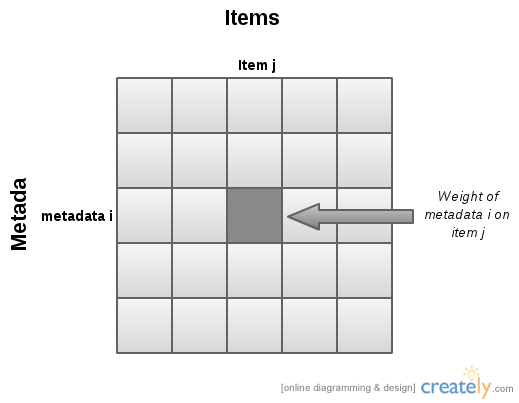
\includegraphics[width=0.7\textwidth]{figures/ICM.png}
    \caption{ICM}
    \label{fig:ICM}
  \end{figure}
 
\item \textbf{User rating matrix}. It's used for collaborative algorithms. It is a matrix which has all the items as columns and all the users as rows. The cell identified by a item and a user contains the rating that the user gave to that movie. It has the value of 0 if there is not any rating for the given item. To better clarify the composition of an user rating matrix, the figure \ref{fig:URM} explains how it is composed.

  \begin{figure}
    \centering
    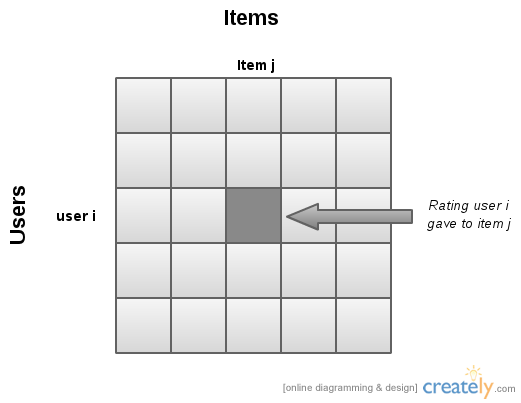
\includegraphics[width=0.7\textwidth]{figures/URM.png}
    \caption{URM}
    \label{fig:URM}
  \end{figure}

The rating can be collected in two different ways:

\begin{itemize}
\item Explicitly. The user is aware that he/she is rating an item. The rating can be provided in different scales. The most common scales are: binary, 3-scale or 5-scale. Binary is a two value rating usually referred as `like` or `dislike`. 3-scale is usually referred as 3 stars or 3 thumbs up. 5-scale is usually referred as 5 stars or a slicer in the 0-5 range. In all the scales, low rating means that the user disliked the item, high values mean that the user liked the item.
\item Implicit. The user is not aware that he/she is rating an item. While browsing the system collect navigation information like clicks on links or displayed pages and based on this information implies ratings for the items. This way of collecting data is very used nowadays with pervasive web applications. Information is key point in business. The more a company know about its customers the better it will be able in satisfy their expectations. 
\end{itemize}
\end{itemize}

\subsection{Stack}
\label{sec:Stack}

To make this possible recommendation system evolved in a stack like way that can be summarized in three phases \cite{sys-rec-matlab}:

\begin{itemize}
\item \textbf{Batch or model creation}. This is a very computational intensive task. Given an ICM or URM it will create a model that will be used later during the recommendation. In this phase most of the computation is performed in order to reduce the computational resources of the next step. Due to the nature of this phase it is seldom run. Usually this kind of operations are run once a week or once a month.
\item \textbf{Real time or recommendation generation}. Given the model elaborated in the previous step and a user or a set of users this task produces the recommendation or a list of items for the user or set of users. The main requirement in this phase is a fast response since it has to run in real-time during page generation. A late response leads in dissatisfaction of the user and a high probability of losing users just because they wait too much the page to be generated. The algorithm should be robust enough to prevent error condition and still gives a valid set of items. 
\item \textbf{Anti reshuffling or recommendation update}. Even after recommendation generation, user can choose a suggested item and thus evaluate it. A good recommendation system is able to react actively under those circumstances and operate in order to generate a new recommendation taking into account the fact that new ratings are added. The new recommendation should thus based on the previous one with small modification. That is why it is called anti reshuffling, to avoid the cycle of the same items.

Figure \ref{fig:Stack} summarize the stack of a recommendation algorithm to better clarify the concept. In the figure there is a clear distinction between what is batch and thus computational intensive and what is not. After that the model is ready the recommendation can be performed which generates the Top N List or the recommendation. 
  \begin{figure}
    \centering
    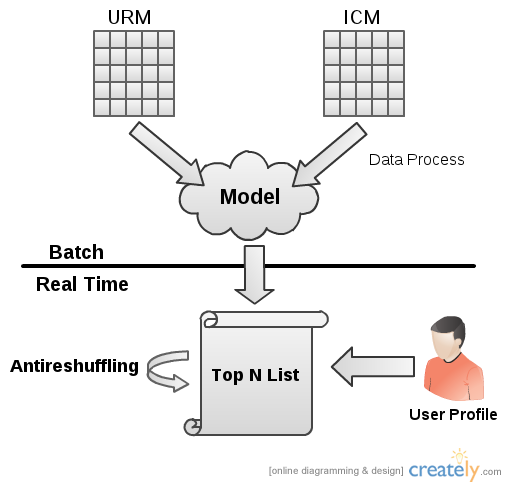
\includegraphics[width=0.7\textwidth]{figures/stack.png}
    \caption{Stack}
    \label{fig:Stack}
  \end{figure}
\end{itemize}

\section{Output}
\label{sec:Output}

As anticipated in the previous section the output of a recommendation system can be of two types:

\begin{itemize}
\item \textbf{Individual scoring}. Given a user the algorithm returns all the rating forecast for this user. This is then turned to a recommendation thanks to the following assumption: recommendation should select items relevant for the user or items that the user will like, since we have user rating forecast we can use the items with the greatest forecasts for our recommendation since the user will probably like them. 
\item \textbf{Top-N recommendation}. The algorithm output a list of the Top-N items most suitable for a certain user. This can also be reproduced starting from the Individual scoring output and ordering that list in descending order of preference..
\end{itemize}

\section{Presentation}
\label{sec:Presentation}

The recommendation algorithm is essential in selecting a relevant subset of items for the user but it's not enough to create a credible recommendation \cite{applicaion-domain-and-functional-classification}. For the recommendation to be useful to the user it must be correctly exposed to the user attention. The way the information is displayed is fundamental and contribute in making a recommendation system successful or not. From recent studies it is also confirmed that the way a recommendation is displayed may affect the items selected by the user \cite{amazon-case}.

Usually recommendation come in a list like form which is a natural way to display a vector of items. A study shows that a text structured overview with concise text and graphics not only facilitates the creation of a trustful relationship between the system and the user but increases user efficiency in selecting a recommended object \cite{trust-building}.

All these studies have been taken in consideration while designing both ContentWise and Milo. They have also been considered in Movish too but the style has been modified taking into account that almost 10 years are passed from that studies and that web application such as Facebook \cite{facebook}, Twitter \cite{twitter} and Pinterest \cite{pinterest} have been gained popularity among users. They provide new ways to explore and display a very big amount of data using a list like, in case of Facebook and Twitter or a catalog like in case of Pinterest, styles. Since movies can be easily represented by their poster which resembles the movie atmosphere, Movish uses a Pinterest like layout to display movie poster, title and genres.

\section{Conclusions}
\label{sec:overview_conclusions}

Recommendation systems are currently a very active research field. The integration with social networks like Facebook, Pinterest, Twitter and Google+ are now opening new ways for them to be more pervasive and be able to match the user tastes better than ever. Also new algorithms are under development that are able to use this new amount of data that was unavailable just five years ago. Not only algorithms and datasets are important, as we demonstrated in this chapter also presentation and usability determine the success or the failure of a recommendation system, especially on e-commerce websites.

Recommendation systems are definitively a kind of technology that will evolve in the future with search engines and other systems in order to increase user satisfaction. In the following chapter we will continue analyzing how Movish has been implemented and how all the challenges that implementing a recommendation system implies have been solved.

\acresetall